% Importante: https://www.sharelatex.com/learn/Theorems_and_proofs
% http://www.inf.pucrs.br/~alfio/ParadigmasFormais/Transition-Systems.pdf - http://home.ufam.edu.br/lucascordeiro/str/slides/02-verificacao-de-modelos.pdf
% Latex math symbols: http://www.ebah.com.br/content/ABAAAAV2MAE/latex-codigos-expressoes-matematicas
% https://www.dimap.ufrn.br/~jair/ES/c2.html - https://felipelirarocha.wordpress.com/2012/04/15/diversos-modelos-de-desenvolvimento-de-software-resumo/ - http://protocoloti.blogspot.com.br/2012/03/os-modelos-de-desenvolvimento-de.html
% http://www.telegraph.co.uk/finance/newsbysector/banksandfinance/11672021/Mobile-banking-has-eclipsed-branches-and-even-the-rest-of-the-internet.html 
% Model Checking: http://ieeexplore.ieee.org/stamp/stamp.jsp?tp=&arnumber=113767
\xchapter{Fundamentação teórica}{}

Este capítulo aborda os principais fundamentos teóricos envolvidos no processo de reparo de refinamento para modelo KMTS.

\section{Desenvolvimento de software}
% falar sobre as fases de desenvolvimento de software

A engenharia de software traz em sua literatura alguns modelos de processos que visam aproximar o cliente dos projetistas de softwares, dentre eles, estão os \textit{modelo em cascata}, \textit{iterativo e incremental}, \textit{prototipação}, \textit{espiral} e etc.

Em um modelo de processo iterativo e incremental a especificação é desenvolvida junto com o software, os clientes identificam em um esboço, as funções a serem fornecidas pelo sistema. Eles identificam quais são as funções mais e menos importantes para eles \cite{sommerville2011engenharia}.
Este tipo desenvolvimento torna-se eficaz na medida em que o cliente ainda não conhece todos os requisitos desejáveis do sistema, o que permite que mudanças possam ocorrer ao longo do processo e que essas mudanças não afete todo o sistema.

O aspecto de desenvolvimento iterativo e incremental proposto pela engenharia de software se encorpora perfeitamente com as técnicas de modelagem formais de software, como por exemplo o \textit{model checking}.

Projetistas de software, geralmente, representam os softwares através de linguagens informais ou semi-formais como UML. Modelos comportamentais de interação se limitam, muitas vezes, a diagrama de sequência \cite{uchitel2003synthesis}.

\section{Model Checking} \label{par-reg}

% - paragrafo falando sobre model checking
% - citar as referencias principais que citam essa técnica
% - descricao formal do que é o model checking
% - ler Baier2008principles e Bérard 2010

A nossa dependência do funcionamento dos sistemas de \textit{Tecnologia da Informação e Comunicação} (TIC) está crescendo rapidamente. Esses sistemas estão se tornando cada vez mais complexos e estão invadindo massivamente nossa vida diária, por meio da Internet e todos os tipos de sistemas embarcados, como \textit{Smart Cards}, \textit{computadores portáteis}, \textit{Smartphones} e \textit{Smart TV} \cite{baier2008principles}.

Com o avanço da tecnologia e com a facilidade do mercado para que cada dia mais e mais pessoas possam adquirir essas novas tenologias, as empresas não só necessitavam desenvolver um software que facilitasse a vida do cidadão, mas precisava garantir ao cliente que o software por ela desenvolvido lhe trouxesse segurança e confiança acima de tudo. Afinal quem gostaria de viajar de avião, se não houvesse uma confiança que o software que roda por trás da máquina é seguro e não tem erros?

% Ler depois http://www.telegraph.co.uk/finance/newsbysector/banksandfinance/11672021/Mobile-banking-has-eclipsed-branches-and-even-the-rest-of-the-internet.html

% - Explicar sobre model checking, o que é e para que serve (se necessário) - %

Para tais problemas existe hoje o model checking. Model Checking consiste na verificação de algumas propriedades do modelo de um sistema.

\section{Modelagem formal de software}

Esse projeto tem como objetivo melhorar o algoritmo de reparo de refinamento desenvolvido por \cite{machado2017uso} e defendido em sua dissertação de mestrado. O modelo formal trabalho por ele foi o KMTS, por permitir mostrar explicitamente determinadas informações parciais de sistema. Para que seja mais fácil o entendimento do que é o reparo de refinamento é necessário falar um pouco sobre o que é refinamento.

\subsection{Estrutura de Kripke}
% Dar uma introdução sobre o que é uma estrutura de kripke e explicar porque ela é importante %
Uma estrutura de Kripke é um modelo matemático útil para descrição de comportamento de sistemas

\theoremstyle{definition}
\begin{definition}
Uma estrutura de Kripke K é uma tupla. $ \mathcal{K} $ = (AP, S, R, L) onde AP é um conjunto de proposições atômicas sobre um estado $\textit{s} \in S$, S é um conjunto de estados, $ R \subseteq S \times S $ uma relação de transição entre os estados e $\textit{L}: \textit{S} \rightarrow 2^{AP}$ uma função de rotuladora.
\end{definition}

% Colocar uma imagem de exemplo de estrutura de kripke e explicar

\subsection{KMTS}

Em um \textit{Kripke Modal Transition Sistem} (KMTS) é interessante notar que ele permite mostrar explicitamente indefinições no sistema.

% Dar uma introdução sobre o que é KMTS %
% Explicar quais são os tipos de indefinições %

\theoremstyle{definition}
\begin{definition}(KMTS \cite{machado2017uso})
Seja AP um conjunto de proposições atômicas e $ Lit = AP \cup \{\neg \textit{p} \; \vert \; \textit{p} \in AP\} $ conjunto de literais sobre AP. Um \textit{Sistema de Transições Modais de Kripke} é uma tupla  $ \mathcal{M} $ = $(AP, S, R^+, R^-, L)$, onde S é um conjunto finito de estados, $ R^+ \subseteq S \times S $ e $ R^- \subseteq S \times S $ são relações de transição tal que $ R+ \subseteq R- $, e $\textit{L}: \textit{S} \rightarrow 2^{Lit}$ é uma função rotuladora, tal que para todo estado $s \in S$ e formula $p \in AP$, pelo menos um entre $\textit{p}$ e $\neg \textit{p}$ ocorre.
\end{definition}

$R^+$ representa as transições \textit{must} (obrigatórias) do sistema e $R^-$ representa as transições \textit{may} (possíveis).

% Colocar uma imagem de exemplo de um KMTS e explicar %

\subsection{Refinamento}

Refinamento se dá na ideia de que dado um objeto ele possui varias versões dele mesmo, uma com mais níveis de detalhes outros com menos, um objeto refinamento do outro se ele tem mais detalhes que o outro objeto analisado. Tomando como exemplo a figura de \cite{machado2017uso}

\begin{figure}[H]
\begin{center}
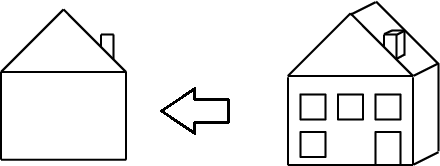
\includegraphics[scale=0.4]{images/refinement1.png}
\caption{Modelo de refinamento}
\label{classificacao-pares}
\end{center}
\end{figure}

a casa B é um refinamento de A, pois, ela possui mais detalhes (menos abstrações), como porta, janelas e chaminés.

Refinamento entre modelos representa uma relação de detalhamento que um modelo tem sobre o outro.


\theoremstyle{definition}
\begin{definition}
abobora
\end{definition}

\subsection{Refinamento de modelo KMTS}

\subsection{Reparo}

\theoremstyle{definition}
\begin{definition}

\end{definition}

\subsection{Reparo de modelo KMTS}

% ----------------------------------------------------------------- %
% | \begin{equation}                                                |
% | A \times B = \{(a,b); a\in A, b\in B\}                          |
% | \end{equation}                                                  |
% |                                                                 |
% | \begin{equation}                                                |
% | M = \{(a,b); a = b, a\in A, b\in B\}                            |
% | \end{equation}                                                  |
% | \begin{equation}                                                |
% | U = \{(a,b); a \neq b, a\in A, b\in B\}                         |
% | \end{equation}                                                  |
% |                                                                 |
% | \begin{equation}                                                |
% | \gamma[\alpha(a),\beta(b)] = \{\gamma^1[\alpha(a),\beta(b)],...,|
% | \gamma^K[\alpha(a),\beta(b)]\}                                  |
% | \end{equation}                                                  |
% ----------------------------------------------------------------- %

% --------------------------- Comentário -------------------------- %

\begin{comment}

\subsection{Método Probabilístico}

Durante o processo de geração dos dados para preenchimento das populações, diferentes tipos de erros podem ser introduzidos nos registros. Dentre eles, destacam-se o preenchimento e/ou codificação diferente dos dados, já que estes são provenientes de fontes diversas, e incompletude dos registros \cite{fellegi1969theory}. O \textit{método probabilístico} constrói, também, um vetor de comparação $\gamma$ com \textit{K} parâmetros
\begin{equation}
\gamma[\alpha(a),\beta(b)] = \{\gamma^1[\alpha(a),\beta(b)], ... , \gamma^K[\alpha(a),\beta(b)]\}
\end{equation} 
sendo esses parâmetros os atributos independentes que serão utilizados para comparação entre os registros \textit{a} e \textit{b}. Isso acontece quando as bases de dados não possuem chaves estrangeiras que consigam relacionar entre si os registros deterministicamente.

Como mostra a figura \ref{classificacao-pares}, eventualmente, existirão casos em que pares verdadeiros negativos sejam classificados no grupo \textit{U}, como também verdadeiros negativos sejam classificados no grupo \textit{M}. São os chamados pares \textit{falsos negativos} e \textit{falsos positivos}.
\begin{figure}[H]
\begin{center}
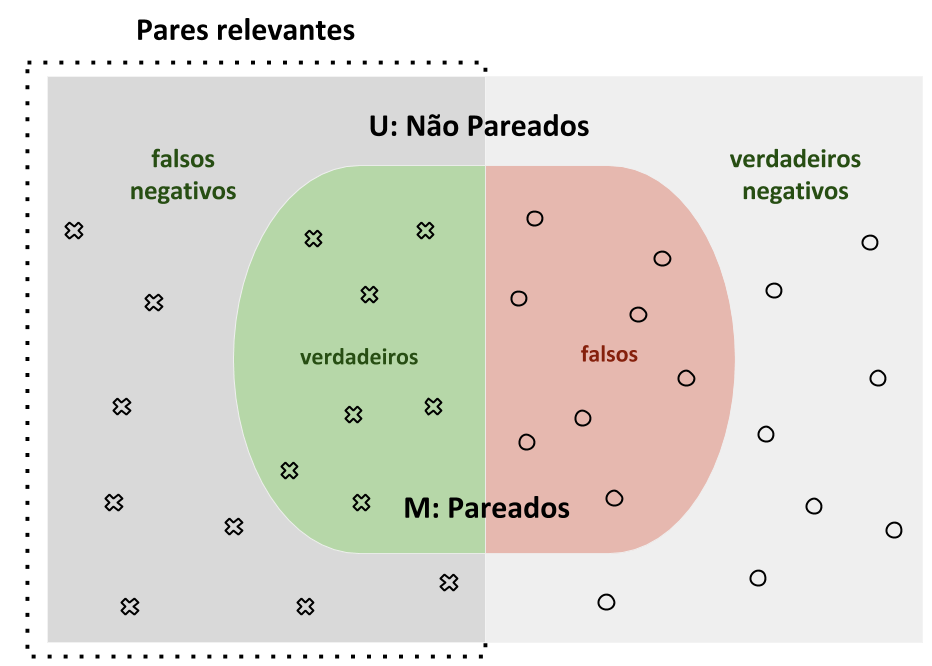
\includegraphics[scale=0.26]{images/pareados_naoPareados.png}
\caption{Classificação dos pares no processo de pareamento probabilístico de registros}
\label{classificacao-pares}
\end{center}
\end{figure}

Essa classificação se dá por conta da inexistência da chave e pela presença de erros nos registros. A \textit{acurácia} do método probabilístico, etapa realizada após o pareamento, é dada a partir das seguintes avaliações:
\begin{enumerate}[a)]
\item $sensibilidade = \frac{verdadeiros\; positivos}{verdadeiros\; positivos\; +\; falsos\; negativos}$
\item $especificidade = \frac{verdadeiros\; positivos}{verdadeiros\; positivos\; +\; falsos\; positivos}$
\end{enumerate}
\begin{figure}[H]
\begin{center}
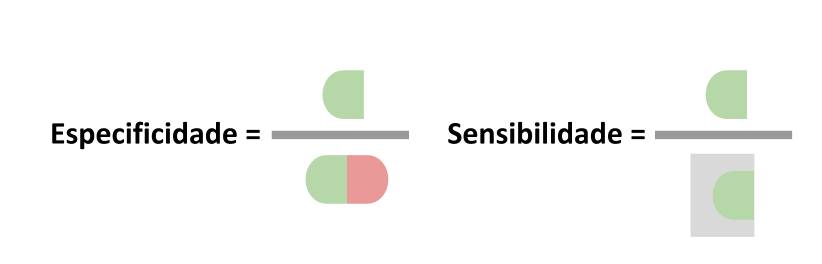
\includegraphics[scale=0.4]{images/sensibilidade_especificidade.png}
\caption{Classificação dos pares no processo de pareamento probabilístico de registros}
\label{classificacao-pares}
\end{center}
\end{figure}

Na prática, o pareamento probabilístico de registros é determinado por funções de similaridade ou distância \cite{kim2007parallel}, denotado por $dist(parametro_1,parametro_2)$, no pseudo-algoritmo abaixo
\begin{algorithmic}
%\STATE $\qquad \qquad para\; cada\; registro\; a_i\; (\in\; A)$
%\STATE $\qquad \qquad \qquad para\; cada\; registro\; b_j\; (\in\; B)$
%\STATE $\qquad \qquad \qquad \qquad se$
\STATE $\qquad\qquad\qquad$ para cada registro $a_i\; (\in A)$
\STATE $\qquad\qquad\qquad\qquad$ para cada registro $b_j\; (\in B)$
\STATE $\qquad\qquad\qquad\qquad\qquad$ se $dist(a_i,b_j) < \Theta$ então $a_i\; \approx\; b_j$
\end{algorithmic}

Quando dois registros, \textit{a} e \textit{b} se referem à mesma entidade no mundo real, é escrito como $a \approx b$. De acordo com \cite{kim2007parallel}, quando esses dois registros são classificados no grupo \textit{M}, quatro relacionamentos, ilustrado na figura X, podem ocorrer: (i) $a \sqsupseteq b$: todas as informações de \textit{b} aparecem em \textit{a}, (ii) $a \sqsubseteq b$: todas as informações de \textit{a} aparecem em \textit{b}, (iii) $a \equiv b$: as informações de \textit{a} e \textit{b} são idênticas, e (iv) $a \oplus b$: parte das informações de \textit{a} e \textit{b} se equivalem além de um \textit{ponto de corte} $\Theta$ determinado. A notação $a \not\approx b$ refere-se quando os registros \textit{a} e \textit{b} não representam a mesma entidade no mundo real ou se as informações referentes à esses registros estão muito abaixo do ponto de corte.
\begin{figure}[H]
\begin{center}
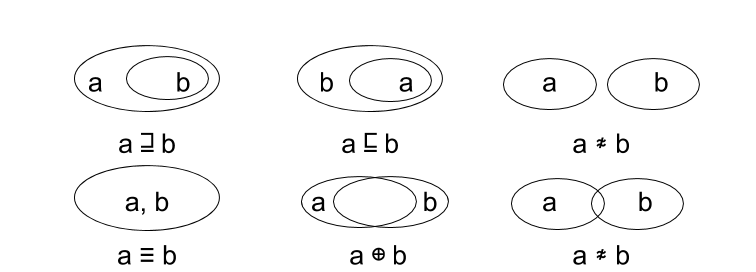
\includegraphics[scale=0.4]{images/relacoes.png}
\caption{Classificação dos pares no processo de pareamento probabilístico de registros}
\label{classificacao-pares}
\end{center}
\end{figure}

\subsection{Filtros de Bloom}

Em muitos bancos de dados, alguns identificadores possuem informações de cunho pessoal, por exemplo: \textit{nome, endereço, referências sobre doença e/ou salário, etc}. Em muitos países, a distribuição e uso para pesquisas científicas de tais bases de dados é um tanto restrita e, por conta disso, é necessário o uso de técnicas de criptografia de dados que consigam tanto garantir o sigilo das informações quanto manter as características necessárias para realização do pareamento. Alguns algoritmos que usam criptografia baseada em funções \textit{hash} conseguem anonimizar as informações e preservar o seu conteúdo, no entanto requerem um pareamento exato dos identificadores. Dessa forma, são ineficientes no \textit{record linkage} quando esses dados possuem diferenças entre si \cite{schnell2009privacy}. Nesse cenário, o \textit{Filtro de Bloom}, método para aproximação de strings, se apresenta como uma alternativa viável.

Inicialmente proposto por \cite{bloom1970space}, o \textit{Filtro de Bloom} é utilizado para determinar se dois elementos são aproximadamente idênticos \cite{jain2005using}. É constituído de um vetor binário \textit{V} de tamanho \textit{n} que inicia todos os seus \textit{bits} com o valor \textit{0}. O objetivo do algoritmo de Filtro de Bloom é armazenar um determinado conjunto $S = \{x_1, x_2,..., x_n\}$, onde cada elemento desse conjunto pode ser caracteres de uma única \textit{string} ou atributos utilizados para o pareamento, em \textit{V}. % Além disso, uma quantidade \textit{k} de funções \textit{hash} $h_1,...,h_k$ são utilizadas para.
Para isso, \textit{k} funções \textit{hash} independentes $h_1,...,h_k$ são %definidas para executar em cada um dos elementos de \textit{S}.
%utilizadas para transformar cada elemento $x_i \in S$ e todos os \textit{bits} que possuem índices $h_j(x_i)$, para $i \leq j \leq k$, tem seus valores mudados para \textit{1}.
utilizadas sobre cada elemento $x_i \in S$ para definir quais posições dentro de \textit{V} terão seu valor alterado para \textit{1}.

Como exemplo, a figura XX exemplifica a atuação do Filtro de Bloom sobre um conjunto \textit{S}, que armazena informações sobre os atributos \textit{nome, município de residência e sexo}.
\begin{figure}[H]
\begin{center}
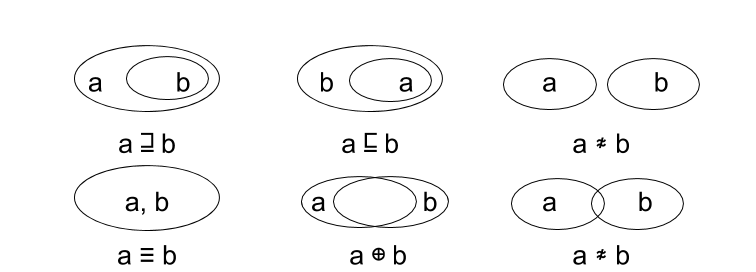
\includegraphics[scale=0.4]{images/relacoes.png}
\caption{Classificação dos pares no processo de pareamento probabilístico de registros}
\label{classificacao-pares}
\end{center}
\end{figure}  

\subsection{Cálculo de Similaridade e Classificação}

No pareamento probabilístico de registros, a etapa de \textit{comparação} dos registros presentes no produto espacial $A \times B$ é baseada no cálculo da probabilidade de concordância e discordância entre os elementos de um determinado par. Essa probabilidade é empregada usando alguma metodologia para verificação de similaridade, principalmente na etapa $\gamma(a,b)$. O \textit{Coeficiente de Dice}, ou Coeficiente de Sorensen-Dice, foi criado para expressar de forma quantitativa, em estudos ecológicos, o grau em que duas espécies distintas estão associadas em diferentes ecossistemas \cite{dice1945measures}. Dado duas espécies, \textit{A} e \textit{B}, o autor propõe inicialmente um \textit{índice de associação}, que é obtido a partir da divisão de um número \textit{a} de amostras aleatórias de uma dada série em que a espécie \textit{A} ocorre por um número \textit{h} de amostras nas quais as espécies \textit{A} e \textit{B} ocorrem em conjunto:
\begin{equation}
Indice\; de\; associacao\; B/A\; = \frac{h}{a}
\end{equation}
\begin{equation}
Indice\; de\; associacao\; A/B\; = \frac{h}{b}
\end{equation}

O Coeficiente de Dice é gerado a partir dos índices de associação e possui um valor intermediário entre os dois índices de associação:
\begin{equation}
Coeficiente\; de\; Dice\; = \frac{2h}{a + b}
\end{equation}
onde (i) \textit{h} representa o somatório dos números de espécies \textit{a} e \textit{b} que coincidem entre si, (ii) \textit{a} corresponde ao número de ocorrências de uma determinada espécie \textit{A}, e (iii) \textit{b} corresponde ao número de ocorrências de uma determinada espécie \textit{B}. Essa técnica pode ser aplicada no contexto do pareamento de registros para uso como coeficiente de similaridade entre dados de bases diferentes, sendo \textit{a} e \textit{b} contadores de um determinado carácter nos Filtros de Bloom \textit{A} e \textit{B}, respectivamente. A figura XX exemplifica como o Coeficiente de Dice realiza o cálculo de similaridade entre dois filtros.
\begin{figure}[H]
\begin{center}
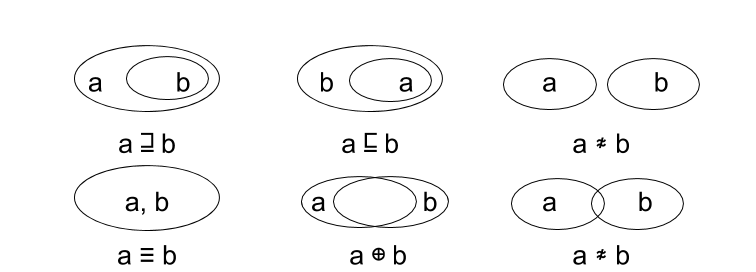
\includegraphics[scale=0.4]{images/relacoes.png}
\caption{Classificação dos pares no processo de pareamento probabilístico de registros}
\label{classificacao-pares}
\end{center}
\end{figure}  

\section{Computação de Alto Desempenho}

Em 1988, um artigo do \textit{Wall Street Journal}, intitulado \textit{Attack of the Killer Micros}, descreveu como os computadores \textit{commodities}, ou computadores pessoais (PCs, do inglês \textit{Personal Computers}), poderiam ser equivalentes aos supercomputadores. De fato, existem casos em que um agrupamento de computadores pessoais pode alcançar níveis de desempenho próximos ou equivalentes aos níveis de um supercomputador, já que há muito mais tecnologias sendo desenvolvidas com a finalidade de melhorar o desempenho de tais computadores do que os supercomputadores. Além disso, o mercado dos PCs se mostrou extremamente promissor com o surgimento de aplicações empresariais, jogos, sistemas multimídia, entre outras. A computação de alto desempenho (HPC, do inglês \textit{High-Performance Computing}) se refere ao uso de supercomputadores ou \textit{clusters} de vários computadores \textit{commodities} no intuito de agregar desempenho para acelerar aplicações que quererem grandes recursos computacionais. 
% - como agregar poder computacional para acelerar aplicacoes, etc.
% - falar das diversas aplicacoes que fazem uso da CAD. falar especificadamente da aplicacao cientifica
% - 


\subsection{Conceitos na Computação Paralela} \label{comp-paralel}

% falar sobre a lei de moore
% falar sobre o aquecimento dos computadores
% falar sobre como esse aquecimento levou ao desenvolvimento de alternativas, uma delas foi o uso de paralelismo (ao nível de instrução e ao nível de threads)

Segundo a \textit{Lei de Moore}, o número de transístores em um circuito eletrônico dobraria a cada dezoito meses sem que os custos de produção aumentassem \cite{moore1998cramming}. Essa lei se tornou a base norteadora das metas de produção dos processadores pelas grandes fabricantes. No entanto, ao passo que a predição de Moore se mostrava acertada, o espaço disponível para inserção desses transístores diminuía e o nível de consumo de energia, implicado pelas altas taxas do \textit{clock}, aumentava. Tornava-se cada vez mais complexo contornar os problemas de dissipação térmica produzida pelos componentes do \textit{hardware}. %Aumentou-se, também, a dificuldade para contornar os problemas de dissipação térmica produzida pelos componentes do hardware. 

Nesse cenário, surgiu as \textit{arquiteturas de computação paralela} \cite{vajda2011multi}, comumente conhecidas como \textit{arquiteturas multicore} (exemplificada na figura \ref{cpu_dual_core}), onde um processor com diversos núcleos (\textit{cores}) explora técnicas de paralelismo, tanto em nível de instruções (ILP - \textit{Instruction-level Parallelism}) quanto em nível de \textit{threads} (TLP - \textit{Threads-level Parallelism}), \textit{pipelining} e processamento com \textit{hyperthreading} \cite{marr2002hyper}. Essas arquiteturas \textit{multicore} possuem dois, quatro, seis ou mais núcleos de processamento. Seguindo essa linha de raciocínio, poderiam incluir centenas de núcleos, no entanto, devido às altas frequências necessárias ao funcionamento de tais arquiteturas, o calor gerado seria excessivo. %geraria um calor excessivo devido às altas frequências necessárias ao funcionamento de tais arquiteturas CITAR. 
A partir disso, surgiram as arquiteturas \textit{manycore}, que tem como base as unidades de processamento gráfico (GPU), compostas de centenas de processadores capazes de explorar o paralelismo em nível de dados (\textit{DLP - Data-level Parallelism}).

\begin{figure}[H]
\begin{center}
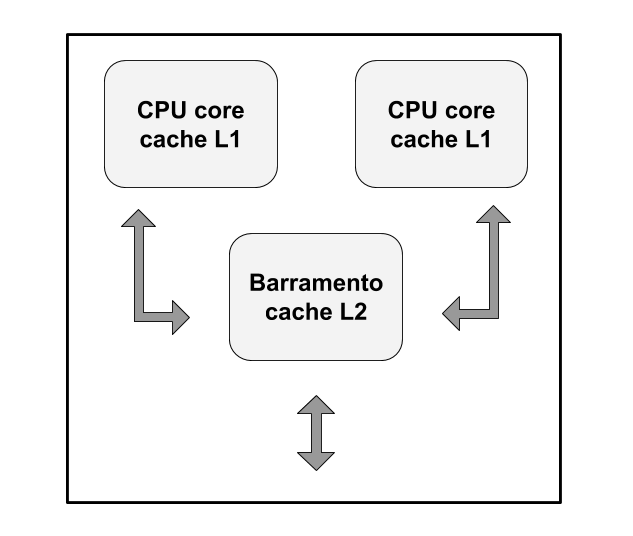
\includegraphics[scale=0.3]{images/cpu_dual_core.png}
\caption{Visão genérica da organização de um processador \textit{dual-core} com memória \textit{cache} interna e compartilhada}
\label{cpu_dual_core}
\end{center}
\end{figure}

%Utilizando a técnica \textit{dividir para conquistar}, onde parte de um problema pode ser executada, de forma paralela, nos múltiplos núcleos presentes nessa arquitetura, os computadores \textit{multicore} tem se mostrado eficientes no aumento do poder computacional e, por consequência, na resolução de problemas que possuem alta complexidade.

Antes do surgimento dessas arquiteturas, os softwares eram projetados para serem executados em um único \textit{core}. Após a introdução das arquiteturas \textit{multicore} e a adoção dessa por parte das aplicações, alguma mudanças ocorreram no processo de desenvolvimento de software e hardware: (i) surgiu a necessidade de se implementar novas técnicas de gerenciamento e comunicação entre os recursos do computador e, principalmente, (ii) mudou-se o paradigma utilizado para o desenvolvimento das aplicações, passando a ser utilizado o paradigma da \textit{programação paralela}. Como consequência, os desenvolvedores passaram a necessitar de um conhecimento mais aprofundado das novas arquiteturas para poderem extrair o máximo de desempenho. Abaixo é listado alguns conceitos presentes na computação paralela.

\begin{itemize}
\item \textbf{Paralelismo:} múltiplos \textit{threads} executando uma tarefa simultaneamente
\item \textbf{Concorrência:} duas aplicações são ditas concorrentes quando estas precisam acessar um recurso compartilhado, uma informação na memória, por exemplo, ao mesmo tempo
\item \textbf{Programação paralela:} técnicas de programação para uso de múltiplos \textit{cores} ou múltiplos computadores
\item \textbf{Computação \textit{multicore}:} computação com sistemas que proveem múltiplos circuitos computacionais por CPU
\item \textbf{Computação distribuída:} computação com sistemas que consiste em múltiplos computadores conectados por uma rede de comunicação
\item \textbf{Paralelismo em nível de instrução:} um programa consiste em um fluxo de instruções executadas pelo processador. Reordenar e combinar em grupos as intruções para que sejam executadas em paralelo sem que altere o resultado final do programa é conhecido como paralelismo em nível de instrução
\item \textbf{Paralelismo em nível de \textit{threads}:}
\item \textbf{Paralelismo em nível de dados:} o mesmo processamento é aplicado à um grande conjunto de dados em paralelo
\item \textbf{Passagem de memória:} modelo de comunicação entre processos onde esta é executada na forma de operações do tipo \textit{send} e \textit{receive}. A comunicação pode ser tanto síncrona, onde o receptor deve estar pronto para receber a mensagem, ou assíncrona, onde a mensagem pode ser enviada antes do receptor estar pronto para recebê-la \cite{el2005advanced}%comunicação com operações básicas (do tipo \textit{enviar} e \textit{receber}, para transmitir informações de um computador para outro
\item \textbf{Memória compartilhada:} modelo de memória que pode ser acessada, tanto para escrita quanto para leitura, simultaneamente por múltiplos \textit{threads} e/ou processos, tendo como objetivo principal prover comunicação entre eles \cite{el2005advanced}. Esse modelo deve prover também controle de acesso, sincronização e proteção dos dados
\end{itemize}

%Com o surgimento do paradigma da computação paralela e no seu uso massivo por grande parte das aplicações, afim de se extrair o máximo de desempenho dos computadores, algumas mudanças ocorreram: (i) ao invés de tentar colocar mais transistores nos componentes eletronicos, mudou-se a arquitetura e passou-se a fabricar computadores com mais de um processador (a exemplo da figura \ref{cpu_dual_core}), (ii) foi necessário implementar novas formas de gerenciar os recursos da máquina, já que [CARACTERISTICAS DO PARALELISMO] passaram a estar presente nas aplicações, e (iii) mudou-se a forma de implementar os softwares, passando a ter como princípio a \textit{programação paralela}.

%A implementação de códigos paralelos consiste basicamente em múltiplos \textit{threads} executando simultaneamente. Esses \textit{threads} associados devem rodar em um mesmo nó pois, na programação paralela, a \textit{memória principal (RAM)} é utilizada como forma de comunicação entre eles. O uso de memória compartilhada é uma das características principais desse paradigma de programação. A outra característica extremamente importante é o uso eficiente das CPUs por um processo. Para isso, desenvolveu-se várias técnicas de paralelismo, tais como: paralelismo a nível de \textit{threads}, a nível de instrução.
%Grande parte das aplicações, atualmente, fazem uso do paradigma da computação paralela para resolver seus problemas. Isso implica na adoção de alguns conceitos impostos no surgimento desse novo paradigma, a fim de extrair o máximo de desempenho dos computadores. Apesar da grande quantidade de ferramentas existentes para a construção de softwares que rodam em paralelo, em linhas gerais, todas elas implementam características como: (i) compartilhamento de memória, (i) gerenciamento de recursos do sistema para \textit{jobs} paralelos

%No entanto, quanto mais transistores se inseria nos circuitos, maiores eram as dificuldades para contornar os problemas de dissipação térmica, além de que o aumento da frequência de \textit{clock} dos processadores já não eram tão visíveis. Nesse cenário, surgiu as \textit{arquiteturas multicore} ou \textit{arquiteturas de computação paralela} a fim de suprir as incessantes buscas pelo aumento da capacidade computacional. Com o advento dessas arquiteturas,     

\subsection{Computação para Multicore}

Com a mudança da arquitetura dos computadores, passando de monoprocessado para multiprocessado, diversas ferramentas de programação paralela surgiram com o objetivo de prover abstrações na exploração eficiente dos recusos de tais arquiteturas. Tanto ferramentas desenvolvidas pelos fabricantes de \textit{software}, quanto de código aberto oferecem aos desenvolvedores de software bibliotecas para os diversos modelos de arquiteturas. No contexto da computação para \textit{multicore}, destacam-se o MPI (\textit{Message Passing Interface}) e o OpenMP (\textit{Open Multi-Processing}).

\subsubsection{MPI} é um padrão industrial que utiliza a troca de mensagem como a principal forma de comunicação entre os processos \cite{mpi}. Para realizar tal comunicação entre os processos, o MPI move os dados de um espaço de armazenamento de um processo para o espaço de armazenamento de outro processo e esse trabalho é realizado através de operações, já implementadas, de troca de mensagem, tais como \textit{send} e \textit{receive}. As principais vantagens do estabelecimento de um padrão de troca de mensagens são a \textit{portabilidade} e a \textit{facilidade de utilização}, já que o MPI possui funções que controlam a passagem de mensagem, a exemplo do \textit{socket} \cite{ribeiro2013programaccao}. Isso permite eximir o programador de obter esse conhecimento.

\subsubsection{OpenMP} é uma API que oferece suporte para a programação paralela. Para isso, possui diretivas de compilação, funções provenientes da biblioteca padrão e variáveis de ambiente que, em conjunto com a memória compartilhada, possibilitam o desenvolvimento de aplicações em sistemas \textit{multicore} \cite{openmp}. Por possuir compartilhamento de memória, o paralelismo é atingido na utilização do modelo \textit{fork-join} e na criação de múltiplos \textit{threads}, que executaram em determinadas regiões paralelas (ver figura \ref{threads_openmp}).

As \textit{diretivas de compilação} permitem criar regiões paralelas, distribuir o trabalho a ser realizado entre os \textit{threads} criados, controlar o acesso aos dados (especificando se são privados ou compartilhados) e gerir a sincronização desses \textit{threads}. Já as \textit{funções da biblioteca} são responsáveis por definir o número de \textit{threads} que será criado, obter informações sobre os mesmos bem como gerir \textit{locks}. As \textit{variáveis de ambiente} definem, também, a quantidade de \textit{threads} além de controlar o escalonamento e definir o máximo aninhamento de regiões paralelas. Abaixo segue um exemplo de código extraído em \cite{openmp-examples}, na linguagem C, que realiza a soma de dois vetores, armazenando-a em um terceiro vetor, com comentários a seguir.

\begin{algorithm}[H]
\begin{center}
% \small
\vspace{1mm}
\begin{verbatim}
1:    #include <stdio.h>
2:    #include <omp.h>
3:
4:    #define N 10000
5:
6:    int main(int argc, char *argv[]) {
7:        int vetorA[N];
8:        int vetorB[N];
9:        int vetorC[N];
10:
11:       #pragma omp parallel for
12:       {
13:           for (int i = 0; i < N; i++)
14:           vetorC[i] = vetorA[i] + vetorB[i];
15:       }
16:
17:       return 0;
18:   }
\end{verbatim}
\vspace{1mm}
\end{center}
\caption {Exemplo de soma de vetores utilizando a API OpenMP}
\label{alg:soma-openmp}
\end{algorithm}

\begin{itemize}
\item É necessário a inclusão da biblioteca OpenMP (\texttt{omp.h}) presente na linha 2

\item \texttt{\#pragma omp $\langle$nome da diretiva$\rangle$ $\langle$[cláusula, ...]$\rangle$} é o formato padrão de uma diretiva no OpenMP
\item \texttt{\#pragma omp parallel $\langle$[cláusula, ...]$\rangle$} é conhecido como construtor paralelo além de ser a diretiva mais importante do OpenMP, uma vez que é o responsável pela indicação da região do código que será executada em paralelo. Esse é o construtor utilizado na linha 9, em conjunto com a cláusula \texttt{for}
\item Para a compilação, é necessário utilizar um compilador que consiga interpretar os \texttt{\#pragmas}. Para utilizar o \textit{gcc} (\textit{GNU Compiler COllection}), é necessário utilizar a opção \texttt{-fopenmp}
\item Para definir a quantidade de \textit{threads} que será criada, pode-se utilizar a cláusula \texttt{num\underline{\space}threads(\textit{n\underline{\space}th})}, sendo o \texttt{n\underline{\space}th} a quantidade exata de \textit{threads}. Outra opção é utilizar uma variável de ambiente, \texttt{OMP\underline{\space}NUM\underline{\space}THREADS=\textit{n\underline{\space}th}}, no momento da execução do código
\end{itemize}

\begin{figure}[H]
\begin{center}
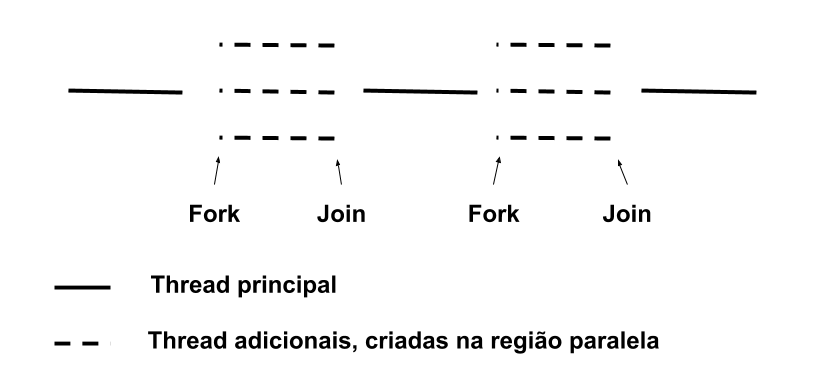
\includegraphics[scale=0.35]{images/threads_openmp.png}
\caption{Modelo \textit{fork-join} para paralelização, utilizado pelo OpenMP}
\label{threads_openmp}
\end{center}
\end{figure}

\subsection{Computação para GPU} \label{comp-gpu}

%Assim como as ferramentas de computação \textit{multicore}, as ferramentas de computação para GPU emergiram no mercado com a intenção 
As unidades de processamento gráfico (GPU) se popularizaram à medida em que aumentou-se o consumo de aplicações que empregavam gráficos 3D, a exemplo dos jogos para computador. Ao perceber a alta demanda por \textit{hardware} que conseguisse processar essas aplicações em específico, a empresa americana NVIDIA lançou sua primeira GPU em 1999, a \textit{GeForce 256} \cite{geforce-256}. Inicialmente, a GPU era constituída de um processador que exercia uma única função: executar aplicações gráficas em três dimensões. Sua característica peculiar é a presença de uma grande quantidade de unidades lógicas (ALU - \textit{Arithmetic Logic Unit}) para processamento do que para \textit{caching} de dados e controle de fluxo, característica das CPUs \cite{boratto2016programaccao} (ver figura \ref{gpu-cpu}). 

Devido à grande capacidade computacional das GPUs, a NVIDIA criou então a GPGPU (\textit{General-Purpose Computing on Graphics Processing Units}), uma GPU de propósito geral capaz de realizar operações complexas da classe SIMD (\textit{Single Instruction Multiple Data}) com extrema facilidade e rapidez. Essas GPUs de propósito geral são divididas em vários SMs (\textit{Streaming Multiprocessors}), onde são executados grupos de \textit{threads}, chamados de \textit{warps}. Vários núcleos, chamados de CUDA \textit{cores}, estão presentes em cada SM e é onde são executadas as operações aritméticas. Esse número considerável de núcleos explica a rapidez com que a GPU executa suas aplicações.

\begin{figure}[H]
\begin{center}
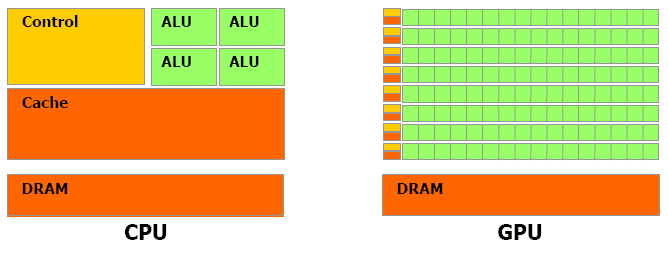
\includegraphics[scale=0.45]{images/gpu_cpu.png}
\caption{Arquitetura de uma CPU \textit{vs} Arquitetura de uma GPU \cite{nvidia-2017}}
\label{gpu-cpu}
\end{center}
\end{figure}

Assim como as ferramentas de computação \textit{multicore}, o surgimento de ferramentas, como DirectX e OpenGL, forneceu aos programadores diversas bibliotecas capazes de extrair o máximo das placas gráficas, permitindo o desenvolvimento de aplicações diversas para serem executadas nessa arquitetura. Um das mais populares é a plataforma CUDA (\textit{Compute Unified Device Architecture}, que será explorada no tópico abaixo.

\subsubsection{CUDA} é uma API que permite o desenvolvimento de software para GPUs, fornecendo abstrações com respeito à organização hierárquica dos \textit{threads}, memória e sincronização. Foi desenvolvida pela NVIDIA e possui suporte a diversas linguagens, dentre elas C/C++. Abaixo são listadas algumas características presentes no desenvolvimento de aplicações com essa API, seguido de um código, extraído de CITAR, exemplificando uma soma de vetores.

\begin{itemize}
\item Ao programar para placas gráficas, é necessário deixar explícito o que será executado na CPU (chamada de \textit{host}) e o que será executado na GPU (chamada de \textit{device}). A função principal a ser executada no \textit{device} recebe o nome de \textit{kernel}

\item Os qualificadores de tipo da função definem quais funções serão executadas no \textit{host} e no \textit{device}. O qualificador \texttt{\_\_global\_\_} define uma função que será executada na GPU e é chamada a partir da CPU, comumente chamada de \textit{kernel}. O qualificador \texttt{\_\_device\_\_} define uma função que será executada na GPU e tem sua chamada a partir da GPU, apenas. Já o qualificador \texttt{\_\_host\_\_} define uma função que é executada somente na CPU.

\item A API CUDA introduz dois novos conceitos para o escalonamento dos \textit{threads}: \textit{bloco} e \textit{grid}. Um bloco é a unidade básica de organização dos \textit{threads} e de mapeamento para o \textit{hardware}, podendo possuir até três dimensões (1D, 2D ou 3D). O \textit{grid} é a unidade básica onde estão distribuídos os blocos e é onde está definido o número total de blocos e de \textit{threads} que serão criados e gerenciados pela GPU, para uma determinada função. Como o bloco, um \textit{grid} pode possuir até três dimensões. A figura \ref{gpu-cpu} exibe a estrutura de um grid de dimensões 2x3 e blocos de tamanho 3x4. Essa API fornece, também, acesso aos índices e dimensões dos \textit{threads}, blocos e \textit{grid}. Cada \textit{thread} possui um índice e este pode ser acessado através da variável \texttt{threadIdx}. Cada bloco dentro do \textit{grid} fornece também um identificador, dado pela variável \texttt{blockIdx}, enquanto que \texttt{blockDim} armazena a dimensão de um bloco de \textit{threads}.

\item Para realizar a computação na GPU, é necessário alocar os dados e transferí-los para o \textit{device}. Isso é feito a partir das funções da API \texttt{cudaMalloc()} e \texttt{cudaMemcpy()}, para alocar e transferir os dados, respectivamente. Após realizar a computação, \texttt{cudaFree()} libera o espaço de memória utilizado na GPU

\item Uma vez alocado e transferido os dados, na chamada de função do \textit{kernel} é necessário informar as dimensões do \textit{grid} e bloco, além dos argumentos que forem necessários para a aplicação. As informações do \textit{grid} e bloco são delimitadas pelos caracteres $<<<$ e $>>>$ e devem ter dimensões compatíveis com o tamanho de entrada do problema.
\end{itemize}

\begin{figure}[H]
\begin{center}
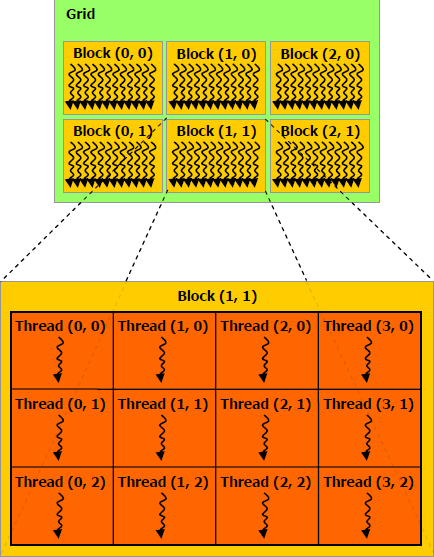
\includegraphics[scale=0.45]{images/grid_blocks.png}
\caption{Organização do \textit{grid} e bloco \cite{nvidia-2017}}
\label{grid-blocks}
\end{center}
\end{figure}

\begin{algorithm}[H]
\begin{center}
% \small
\vspace{1mm}
\begin{verbatim}
1:    #include <stdio.h>
2:    #include <cuda.h>
3:
4:    #define N 100000
5:
6:    __global__ void kernel(int *A, int *B, int *C) {
7:        int i = threadIdx.x;
8:        C[i] = A[i] + B[i];
9:    }
10:
11:   int main() {
12:       int A[N], B[N], C[N];
13:       int *A_device, *B_device, *C_device;
14:       
15:       cudaMalloc((int **) &A_device, sizeof(int) * N);
16:       cudaMalloc((int **) &B_device, sizeof(int) * N);
17:       cudaMalloc((int **) &C_device, sizeof(int) * N);
18:
19:       cudaMemcpy(A_device, A, sizeof(int) * N, cudaMemcpyHostToDevice);
20:       cudaMemcpy(B_device, B, sizeof(int) * N, cudaMemcpyHostToDevice);
21:
22:       // Chamda do kernel com 1 bloco e N threads
23:       kernel<<<1, N>>>(A, B, C);
24:
25:       cudaMemcpy(C, C_device, sizeof(int) * N, cudaMemcpyDeviceToHost);
26:
27:       cudaFree(A_device);
28:       cudaFree(B_device);
29:       cudaFree(C_device);
30:
31:       return 0;
32:   }
\end{verbatim}
\vspace{1mm}
\end{center}
\caption {Exemplo de soma de vetores utilizando a API OpenMP}
\label{alg:soma-openmp}
\end{algorithm}

\begin{itemize}
\item Utilizando a linguagem C, é necessário importar a biblioteca \texttt{cuda.h} da API CUDA (linha 2)

\item Na linha 6 inicia-se a função \textit{kernel}, com o qualificador \texttt{\_\_global\_\_}

\item Como o código manipula um vetor de dimensão 1, utiliza-se o identificador \texttt{threadIdx.x} para notação do índice do vetor. Caso fosse uma matriz (2 dimensões, por exemplo), utilizaria a seguinte notação: \texttt{threadIdx.y} para a segunda dimensão

\item Nas linhas 15, 16 e 17 aloca-se as variáveis na GPU, enquanto que nas linhas 19 e 20 é copiado os dados das variáveis no \textit{host} para as variáveis no \textit{device}

\item A chamada do \textit{kernel} é feita na linha 23, onde são passados a dimensão do \textit{grid} ou quantidade de blocos (no código tem dimensão 1) e a quantidade de \textit{threads} por bloco (no código possui N threads), respectivamente, entre $<<<$ e $>>>$

\item O resultado da computação na GPU é transferida para uma variável do \textit{host} na linha 25, enquanto que é liberado a memória do \textit{device} nas linhas 27, 28 e 29
\end{itemize}

\subsection{Computação heterogênea}

Como explanado nas seções \ref{comp-paralel} e \ref{comp-gpu} desse capítulo, por possuírem um grande número de núcleos de processamento, as GPUs deixaram de ser usadas exclusivamente para processamento gráfico e passaram a suportar aplicações de propósito geral. Assim como as GPUS, as arquiteturas \textit{multicore} tem possibilitado obter um alto ganho de desempenho frente às arquiteturas monoprocessadas. Os avanços no desenvolvimento dessas arquiteturas, mais robustas e paralelizáveis, possibilitaram utilizá-las em conjunto no intuito de prover soluções para problemas que envolvem a computação intensiva, a exemplo de cálculos matemáticos e processamento de grandes bancos de dados.
%se tornaram bastante atrativas quando se deseja prover soluções para problemas que envolvem a computação intensiva (TROCAR ESSA PALAVRA). Assim como as GPUs, as arquiteturas \textit{multicore} tem possibilitado obter um ganho de desempenho em tais aplicações. Os avanços no desenvolvimento dessas arquiteturas, mais robustas e paralelizáveis, possibilitaram utilizá-las em conjunto no intuito de solucionar
Esse uso coordenado das diferentes arquiteturas é denominado \textit{Computação Heterogênea} (HC, do inglês \textit{Heterogeneous Computing}) \cite{maheswaran1999heterogeneous}. Um \textit{cluster} composto por diferentes tipos (modelos ou gerações) de máquinas pode constituir um sistema de computação heterogênea ou, alternativamente, ser tratado como uma simples máquina em um sistema HC mais amplo. 

O autor \cite{braun2001heterogeneous} define que um problema clássico da HC: uma aplicação é composta por uma ou mais tarefas independentes e que algumas dessas tarefas podem ser decompostas em duas ou mais subtarefas. Essas subtarefas possuem dependência de dados entre elas, mas podem ser atribuídas a diferentes máquinas para execução, onde estas possuem algum canal de comunicação. Dado o poder computacional de cada componente do sistema HC e quais tipos de tarefas se comportam melhor em cada um desses, o objetivo é distribuir as subtarefas entre os componentes a fim de obter ganho de desempenho na aplicação (ver figura XX). [poderia falar sobre os desafios da area: comunicacao, arquiteturas diferentes =$>$ balanco de carga, etc]

Além das arquiteturas \textit{multicore} e GPU, os \textit{coprocessadores}, principalmente os baseados na arquitetura Intel MIC (\textit{Many Integrated Core}), tem sido largamente utilizado na computação heterogênea \cite{huang2015study}, sendo adotados no intuito de empregar soluções utilizando o paralelismo para alcançar tanto um alto ganho de desempenho quanto escalabilidade e baixo consumo de energia. A arquitetura geral de um Intel MIC (\textit{Many Integrated Core}), um dos coprocessadores mais utilizados na indústria, é composta de vários núcleos de processamento interligados através de um barramento de alta velocidade. O \textit{Knights Corner}, coprocessador da linha Intel \textit{Xeon Phi} lançado em 2011, possui 61 \textit{cores} de baixo consumo de energia e cada \textit{core} executa quatro \textit{threads} em paralelo. Essa arquitetura utiliza o modelo de memória compartilhada e permite utilizar modelos tradicionais da computação \textit{multicore}, tais como OpenMP.

%O uso coordenado de diferentes tipos de máquinas, arquiteturas, redes e interfaces, com o intuito de maximizar o desempenho combinado entre os dispositivos, é denominado \textit{Computação Heterogênea} (HC, do inglês \textit{Heterogeneous Computing}) \cite{maheswaran1999heterogeneous}. Os avanços no desenvolvimento de arquiteturas de computadores mais robustas e paralelizáveis possibilitaram utilizar uma vasta coleção de máquinas, de \textit{hardware} e \textit{software} diferentes, no intuito de solucionar problemas de natureza intensiva no campo da computação.

%Com os recentes avanços no desenvolvimento de arquiteturas de computadores mais robustas e paralelizáveis, tem sido possível utilizar uma vasta coleção de máquinas e sistemas com diferentes arquiteturas no intuito de prover soluções para diferentes tarefas intensivas na computação. Esse uso coordenado de diferentes tipos de máquinas, redes e interfaces para maximizar o ganho de desempenho aliado à um baixo custo é denominado \textit{Computação Heterogênea} (HC - \textit{Heterogeneous Computing}) . 

\end{comment}